\section{Kinetic Inductance Detectors}
\label{se:kids}
%\subsection{KID physics}

%\begin{figure}[h]
\begin{figure}
\center
	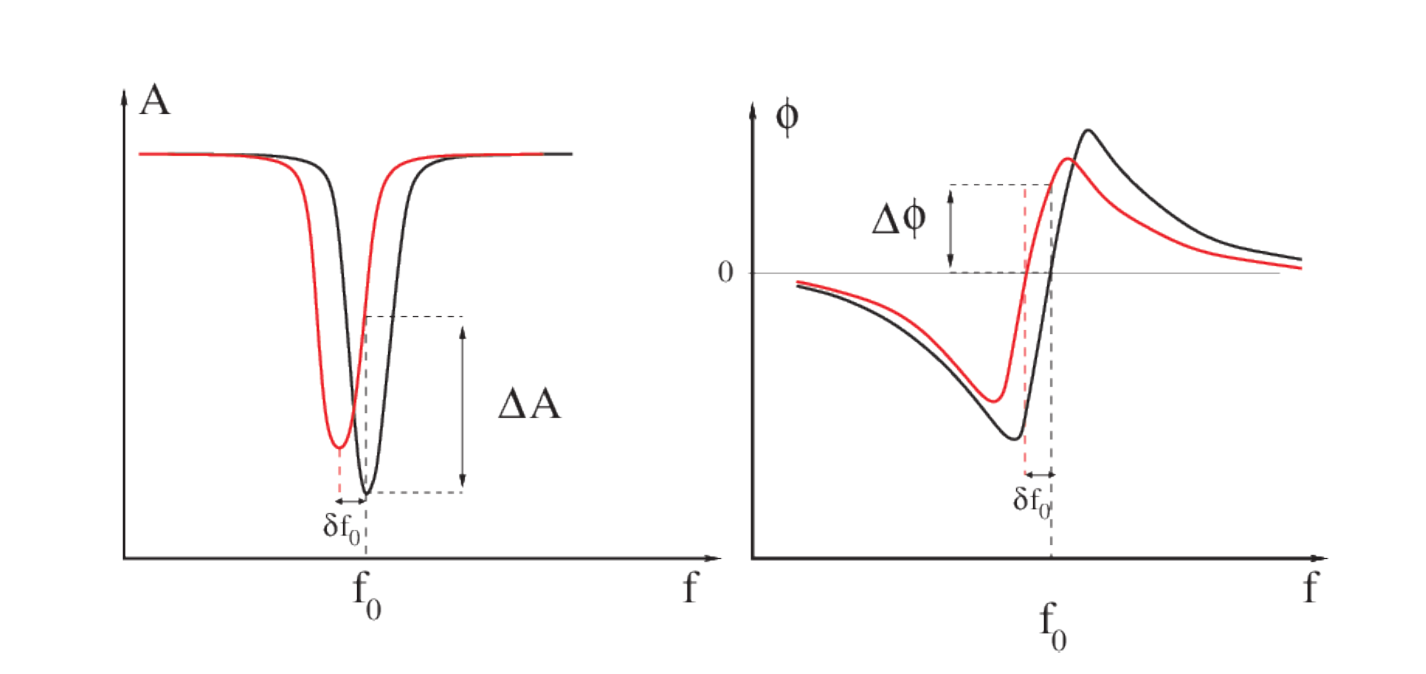
\includegraphics[clip, angle=0, width=\columnwidth]{Figures/resonance.png}
%	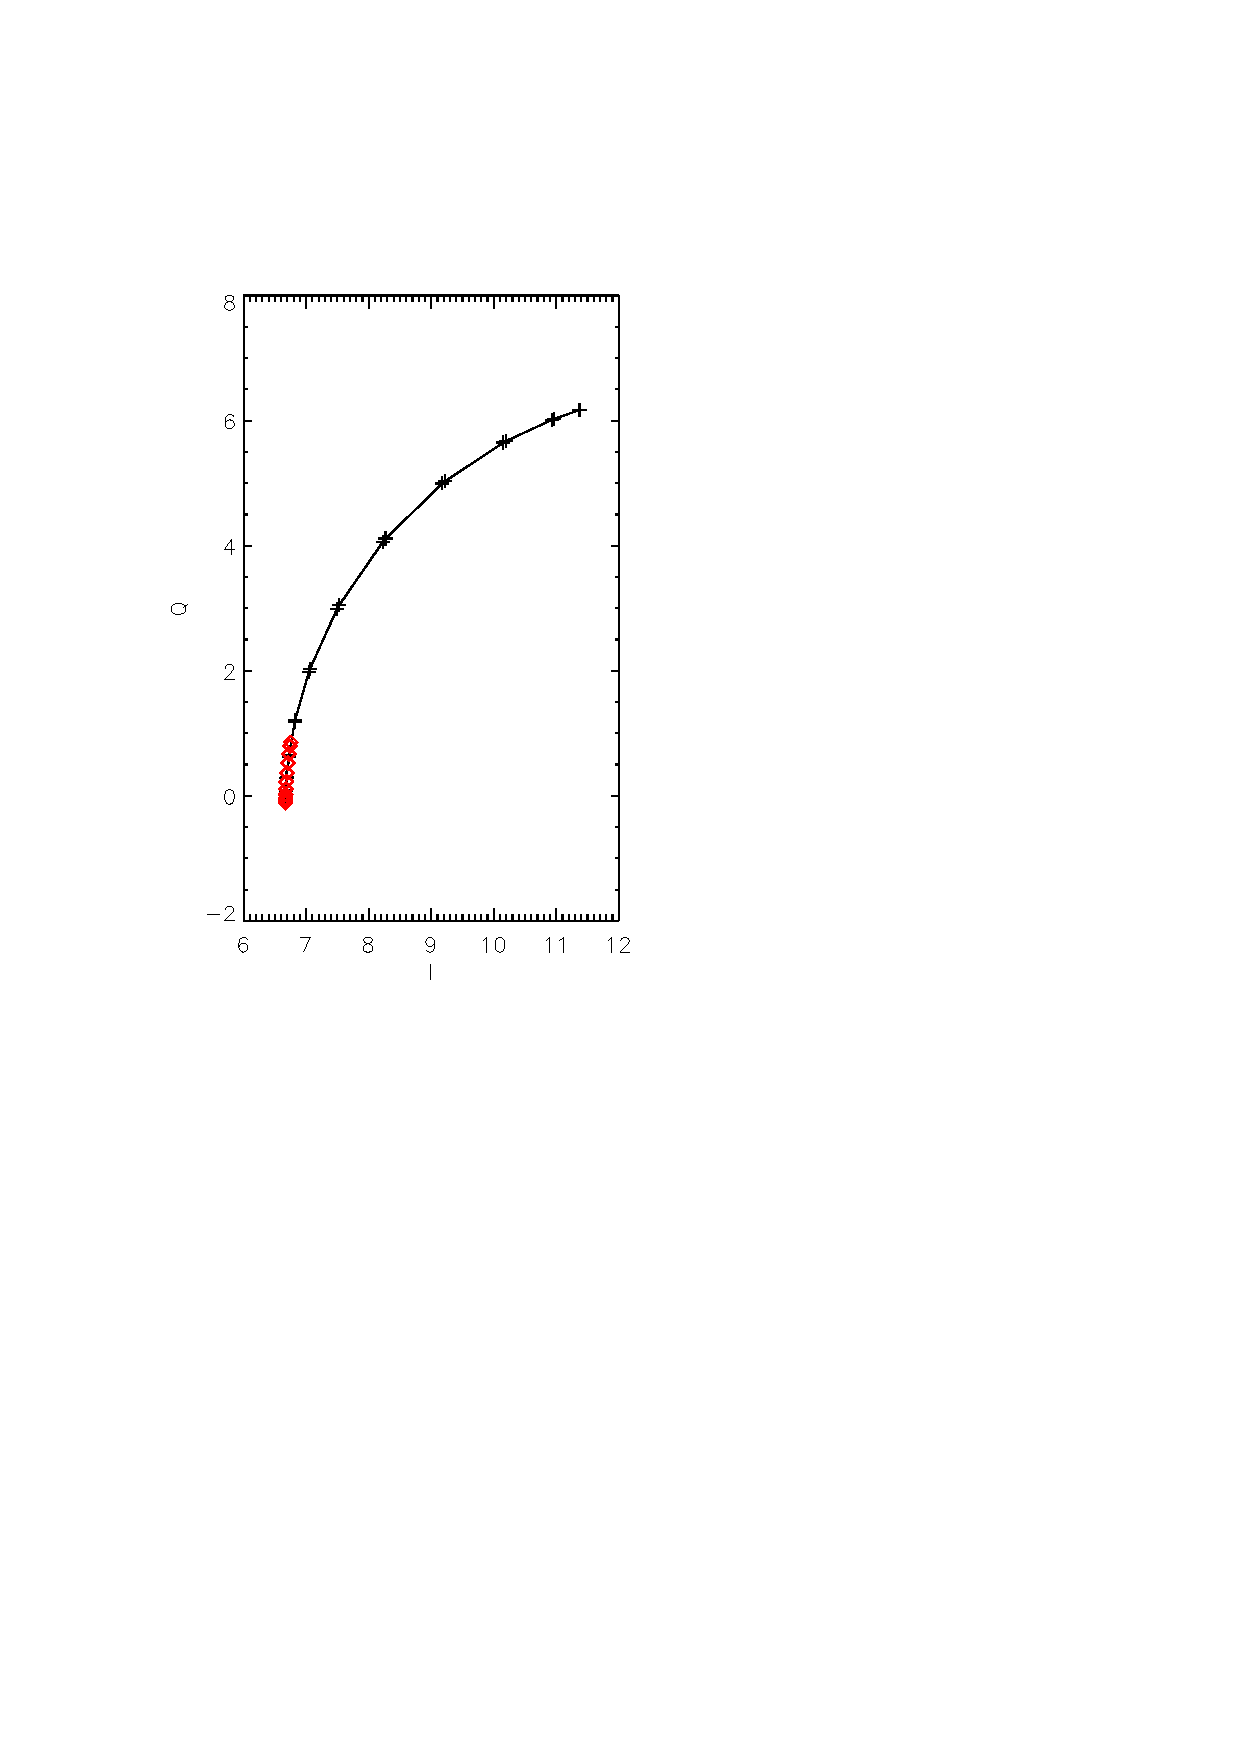
\includegraphics[clip, angle=0, width=\columnwidth]{Figures/resonance.pdf}
	\caption{Schematic representation of a KID resonance in amplitude (left) and phase (right), as a function of the excited tone injected in the feedline. The optical power absorbed by the detector is weak for black curves and increases for red curves. The absorption of a photon shifts the resonance frequency and this is directly proportional to the received power.}
	\label{resonance}
\end{figure}

Kinetic Inductance Detectors (KID) are a novel superconducting detector technology
that provides high sensitivity and ease of multiplexing. In this section we give
a brief summary of their main features and how photometry can be derived from
their measurements.

\subsection{Transfer function}

KIDs are RLC superconducting resonators made from a thin metal film. When
photons are absorbed by the superconducting film, they break Cooper pairs which
increases the quasi-particles density and causes a change in the kinetic
inductance $L_{k}$. This produces a shift $\delta f_{0}$ of the resonant
frequency of the KID \citep{2013A&A...551L..12C} that can be related to the
absorbed optical power $\delta P_{opt}$ (cf.~Fig.~\ref{fig:resonance}). This
relation is linear for small variations in $P_{opt}$
\citep{2010ApPhL..96z3511S}. The KID transfer function is given by:

\begin{equation}
S_{21}(f) = \mathcal{I} +j\mathcal{Q} .
\end{equation}

\noindent where $\mathcal{I}$ and $\mathcal{Q}$ give respectively the real (in phase) and imaginary
(quadrature) of $S_{21}$. A model of a KID transfer function has been proposed
by \citet{2008ApPhL..93m4102G} :

\begin{equation}
S_{21} = \frac{2Z_{res}Z_{0}}{Z_{res}[2Z_{0} + j(X_{1}+X_{2})] + (Z_{0} +jX_{1})(Z_{0} +jX_{2})},
\end{equation}

with:

\begin{equation}
Z_{res} = \frac{Z_{0}Q_{e}}{2Q_{i}}[1 + 2jQ_{i}\frac{(f-f_{0})}{f_{0}}],
\end{equation}

\noindent where $X_{1}$, $X_{2}$, $Z_{0}$ are impedances, $Q_{i}$ is the
intrinsic quality factor of the resonator and $Q_{e}$ is the external quality
factor due to coupling with the measurement electronics. $f$ is the frequency of
excitation of the detector, and $f_{0}$ is the resonant frequency. Throughout
this paper, we shall assume typical values of KIDs $X_{1} = X_{2} =
0.5\,\Omega$, $Z_{0} = 50\,\Omega$, $Q_i=2\times 10^4$, $Q_e=10^4$ and $f_{0} =
1.8\times 10^9$\,Hz as measured on \nika\ and \nikad. The following section
addresses how the resonance of a KID is monitored and related to the incident
optical power.

